\documentclass{beamer}

\useoutertheme[glossy]{wuerzburg}
\useinnertheme[shadow,outline]{chamfered}
\usecolortheme{shark}
\beamertemplatenavigationsymbolsempty 

\usefonttheme{professionalfonts}
\let\digamma\relax
\usepackage[scale=0.85,stdmathitalics=true,romanfamily=casual]{lucimatx}
\usefonttheme[stillsansseriftext]{serif}


\usepackage{fancyvrb}

%% Fancy syntax coloring via pygments
\usepackage{minted}
\definecolor{bg}{rgb}{0.95,0.95,0.95}
\usemintedstyle{borland}


\newenvironment{Rcode}
{\VerbatimEnvironment
 \begin{minted}[fontsize=\scriptsize,baselinestretch=1]{r}}%
{\end{minted}}

\newenvironment{Pcode}
{\VerbatimEnvironment
 \begin{minted}[fontsize=\scriptsize,baselinestretch=1]{python}}%
{\end{minted}}

\newenvironment{Code}[1]
{\VerbatimEnvironment
 \begin{minted}[fontsize=\scriptsize,baselinestretch=1]{#1}}%
{\end{minted}}


\usepackage{textfit} % commands \scaletoheight{height}{text} and \scaletowidth{width}{text}

\usepackage{tikz}


\newtheorem{Alert}{Alert}
\newtheorem{Highlight}{Highlight}

\newcommand{\Species}[1]{{\rmfamily \itshape #1}}
\newcommand{\Real}{\ensuremath{\mathbb{R}}}
\newcommand{\RealN}{\ensuremath{\mathbb{R}^n}}
\newcommand{\RealP}{\ensuremath{\mathbb{R}^p}}
\newcommand{\Mtx}[1]{\ensuremath{\mathbf{#1}}}
\newcommand{\Inv}[1]{\ensuremath{#1^{-1}}}
\newcommand{\InvMtx}[1]{\ensuremath{\mathbf{#1}^{-1}}}
\newcommand{\Red}[1]{\textcolor{red}{#1}}
\newcommand{\PsInv}[1]{\ensuremath{\mathbf{#1}^{+}}}



\usepackage{tikz}
\usepackage{marvosym} % for male/female symbols
\usepackage{MnSymbol} % for thinstar

\setbeamersize{description width=2em}

\DeclareMathOperator{\rank}{rank} 

%===========================================================
% Title Info
\title{Scientific Computing for Biologists}
\subtitle{Singular Value Decomposition and Biplots}

\author{Instructor: Paul M. Magwene}


\date{18 October 2011}

\begin{document}
%===========================================================
\begin{frame}
\titlepage
\end{frame}

%===========================================================
\begin{frame}
  \frametitle{Overview of Lecture}
  
\begin{itemize}
		\item Singular Value Decomposition
		\begin{itemize}
			\item Algebra of SVD
			\item Geometry of SVD
			\item Relationship to Eigendecomposition
			\item Applications of SVD			
		\end{itemize}		
		\item Biplots
		\begin{itemize}
			\item Simultaneous representation of rows and columns of a matrix
		\end{itemize}			
\end{itemize}

\end{frame}
%===========================================================

%===========================================================
\begin{frame}
  \frametitle{Hands-on Session}
\begin{itemize}
    \item SVD and Biplots in R
    \item SVD in Python
    \item Applications of SVD in R and Python
    		\begin{itemize}
    		\item `Seriation' using SVD
			\item Matrix approximation and image compression using SVD
		\end{itemize}
\end{itemize} 


\end{frame}		
%===========================================================


%===========================================================
\begin{frame}
  \frametitle{Eigendecomposition}

$$ \Mtx{A} = \Mtx{U}\Mtx{D}\InvMtx{U} $$

where:
\begin{itemize}
\item  $\Mtx{U}$ is a matrix of eigenvectors (in columns)
\item $\Mtx{D}$ is a diagonal matrix with eigenvalues along diagonal.
\end{itemize}

\medskip
when $\Mtx{A}$ is real-valued and symmetric than $\Mtx{U}$ is orthgonal.

\end{frame}
%===========================================================

%===========================================================
\begin{frame}
  \frametitle{Singular Value Decomposition}


%$$ \Mtx{A} = \Mtx{U}\Mtx{S}\Mtx{V}^T $$

\begin{center}
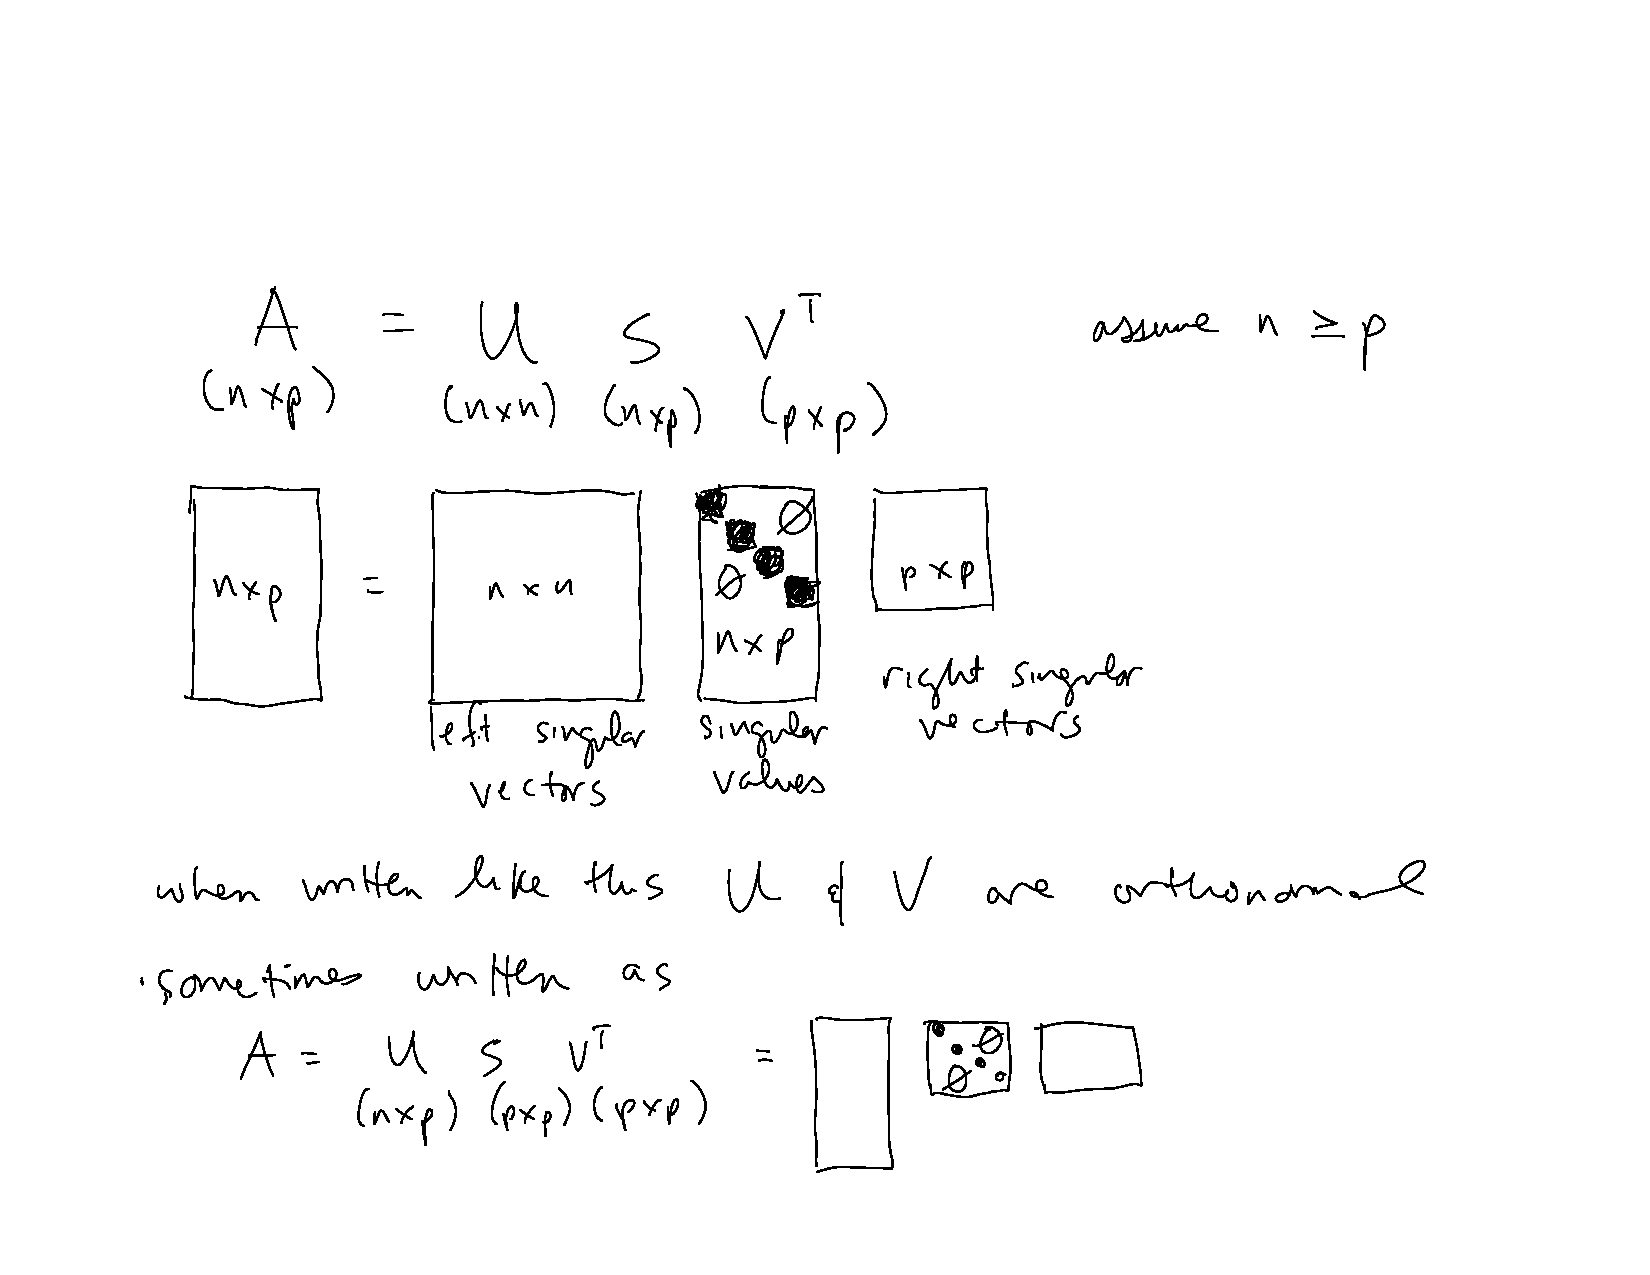
\includegraphics[height=3in]{svd-graphic}
\end{center}

\end{frame}
%===========================================================


%===========================================================
\begin{frame}
  \frametitle{Facts about SVD}

\begin{itemize}
\item Singular Value Decomposition is often referred to as giving the ``basic structure'' of a matrix

\item The rank of $\Mtx{A}$ is equivalent to the number of non-zero singular values in $ \Mtx{A} = \Mtx{U}\Mtx{S}\Mtx{V}^T $

$$ \rank(\Mtx{A}) \leq \min(n,p) $$


\item  The Euclidean norm ($L_2$) norm of a matrix is the relative amount it stretches a vector:

$$ |\Mtx{A}|_E = \frac{|\Mtx{A}\Mtx{x}|}{|\Mtx{x}|} $$

The $L_2$ norm of $\Mtx{A}$ is given by $\Mtx{S}_{11}$.
\end{itemize}



\end{frame}
%===========================================================

%===========================================================
\begin{frame}
  \frametitle{Geometric Interpretation of SVD}

Any matrix, $\Mtx{A}_{n \times p}$, represents a linear transformation from $\RealP \mapsto  \RealN$. 

\medskip
SVD can be thought of decomposing the transformation specified by $\Mtx{A}$ into a simple form:

$$ \Mtx{A} = (\text{rotation})(\text{scaling)}(\text{rotation})$$

\begin{itemize}
\item $\Mtx{U}$ and $\Mtx{V}$ are orthonormal matrices $\rightsquigarrow$ Orthonormal matrices represent rigid rotations (or rotation plus reflection)
\item Diagonal matrices represent ``stretching''
\end{itemize}


\end{frame}

%===========================================================


%===========================================================
\begin{frame}
  \frametitle{SVD Example}

\begin{center}
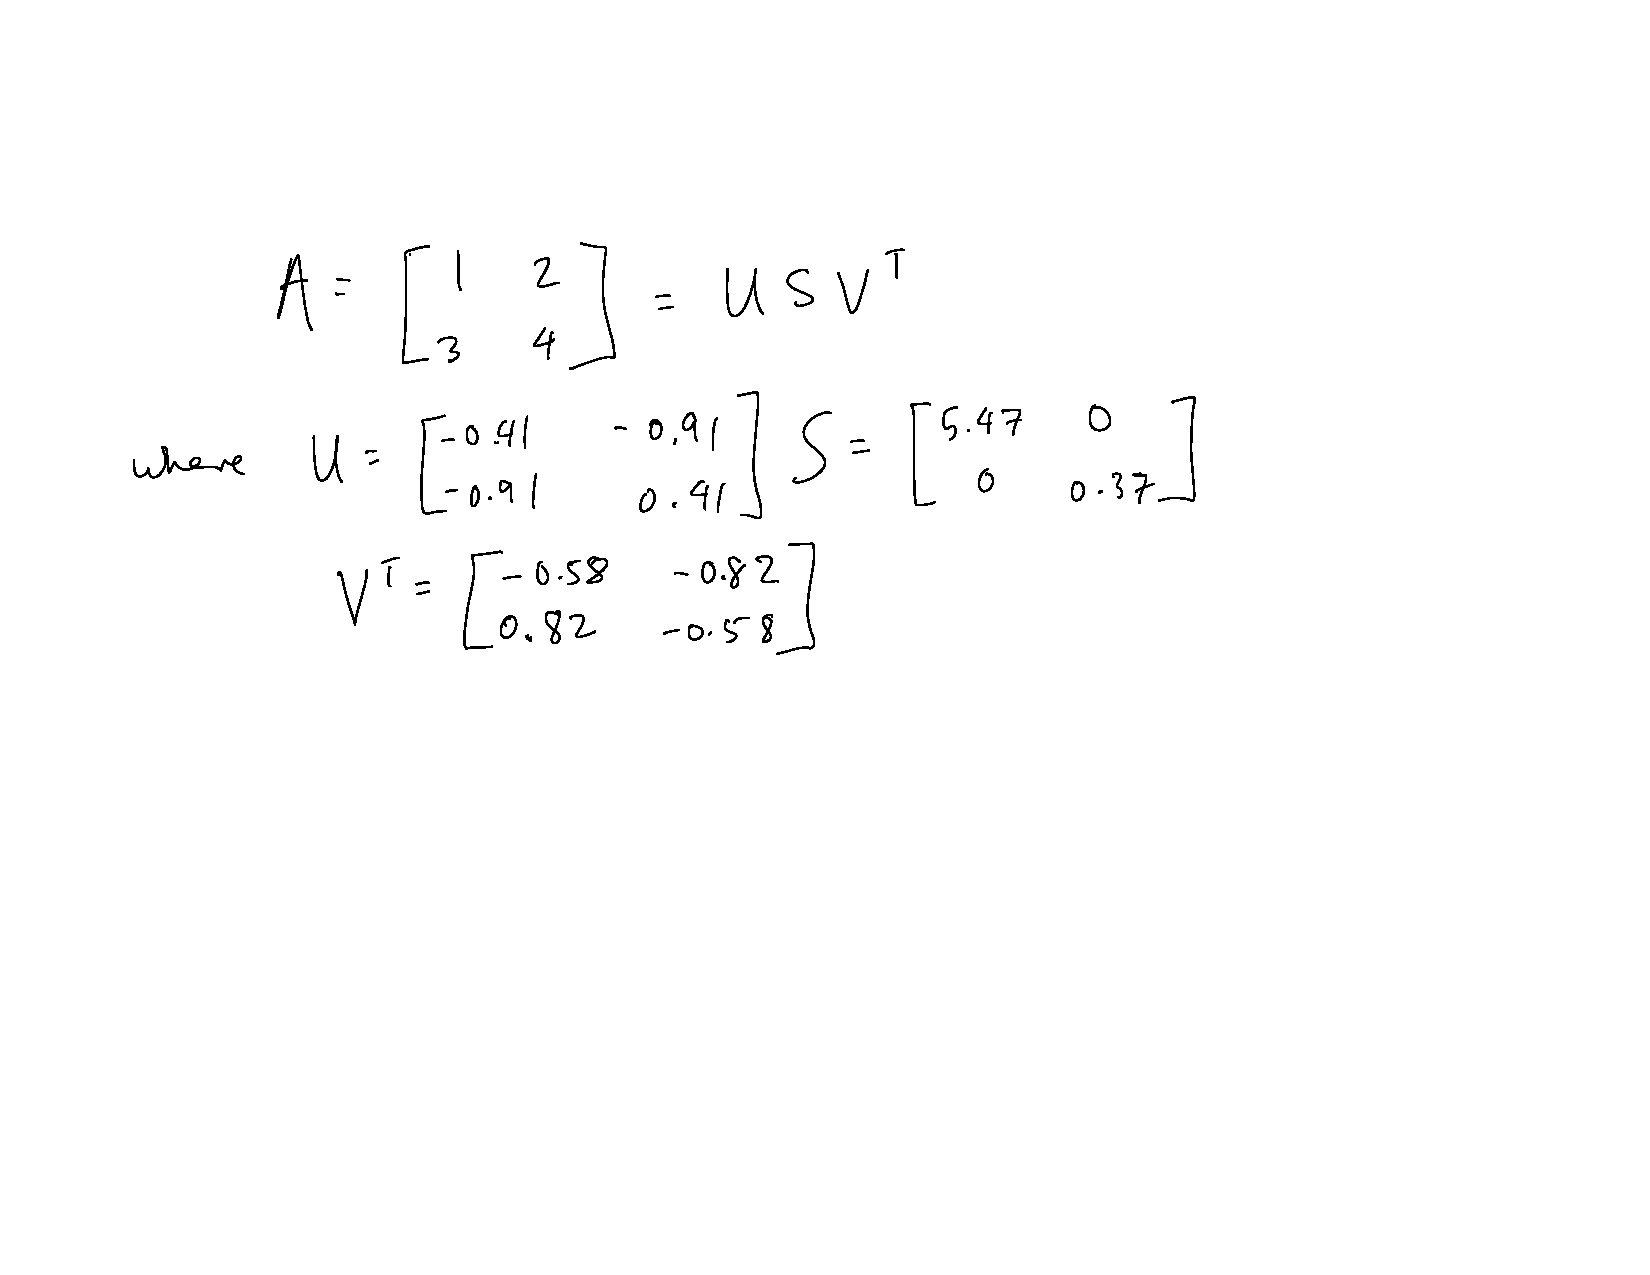
\includegraphics[height=1.25in]{svd-example-mtx}
\end{center}

\medskip
\textbf{Geometry}
\begin{center}
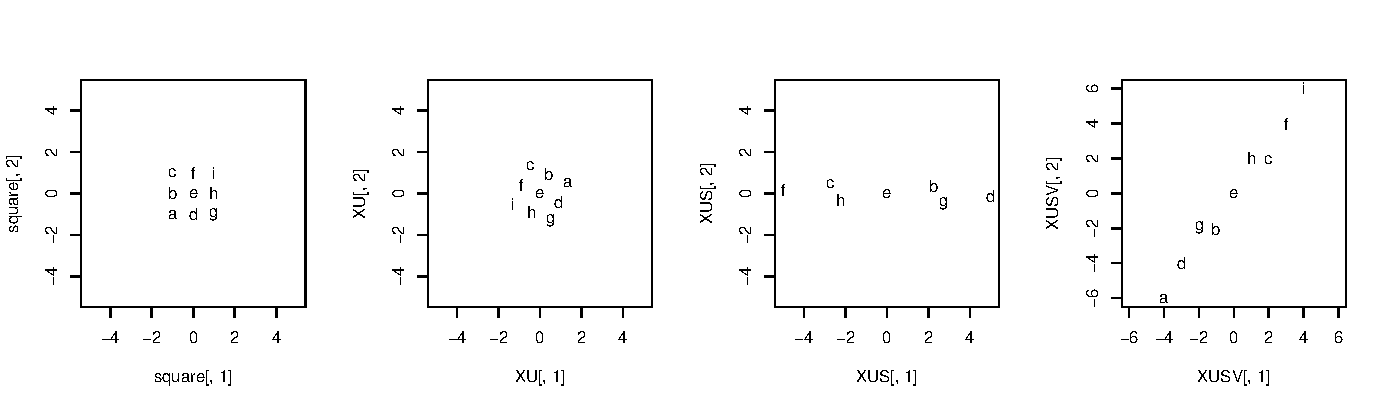
\includegraphics[height=1.25in]{svd-example}
\end{center}

\end{frame}
%===========================================================


%===========================================================
\begin{frame}
  \frametitle{Relationship of SVD to Eigendecomposition}

\begin{center}
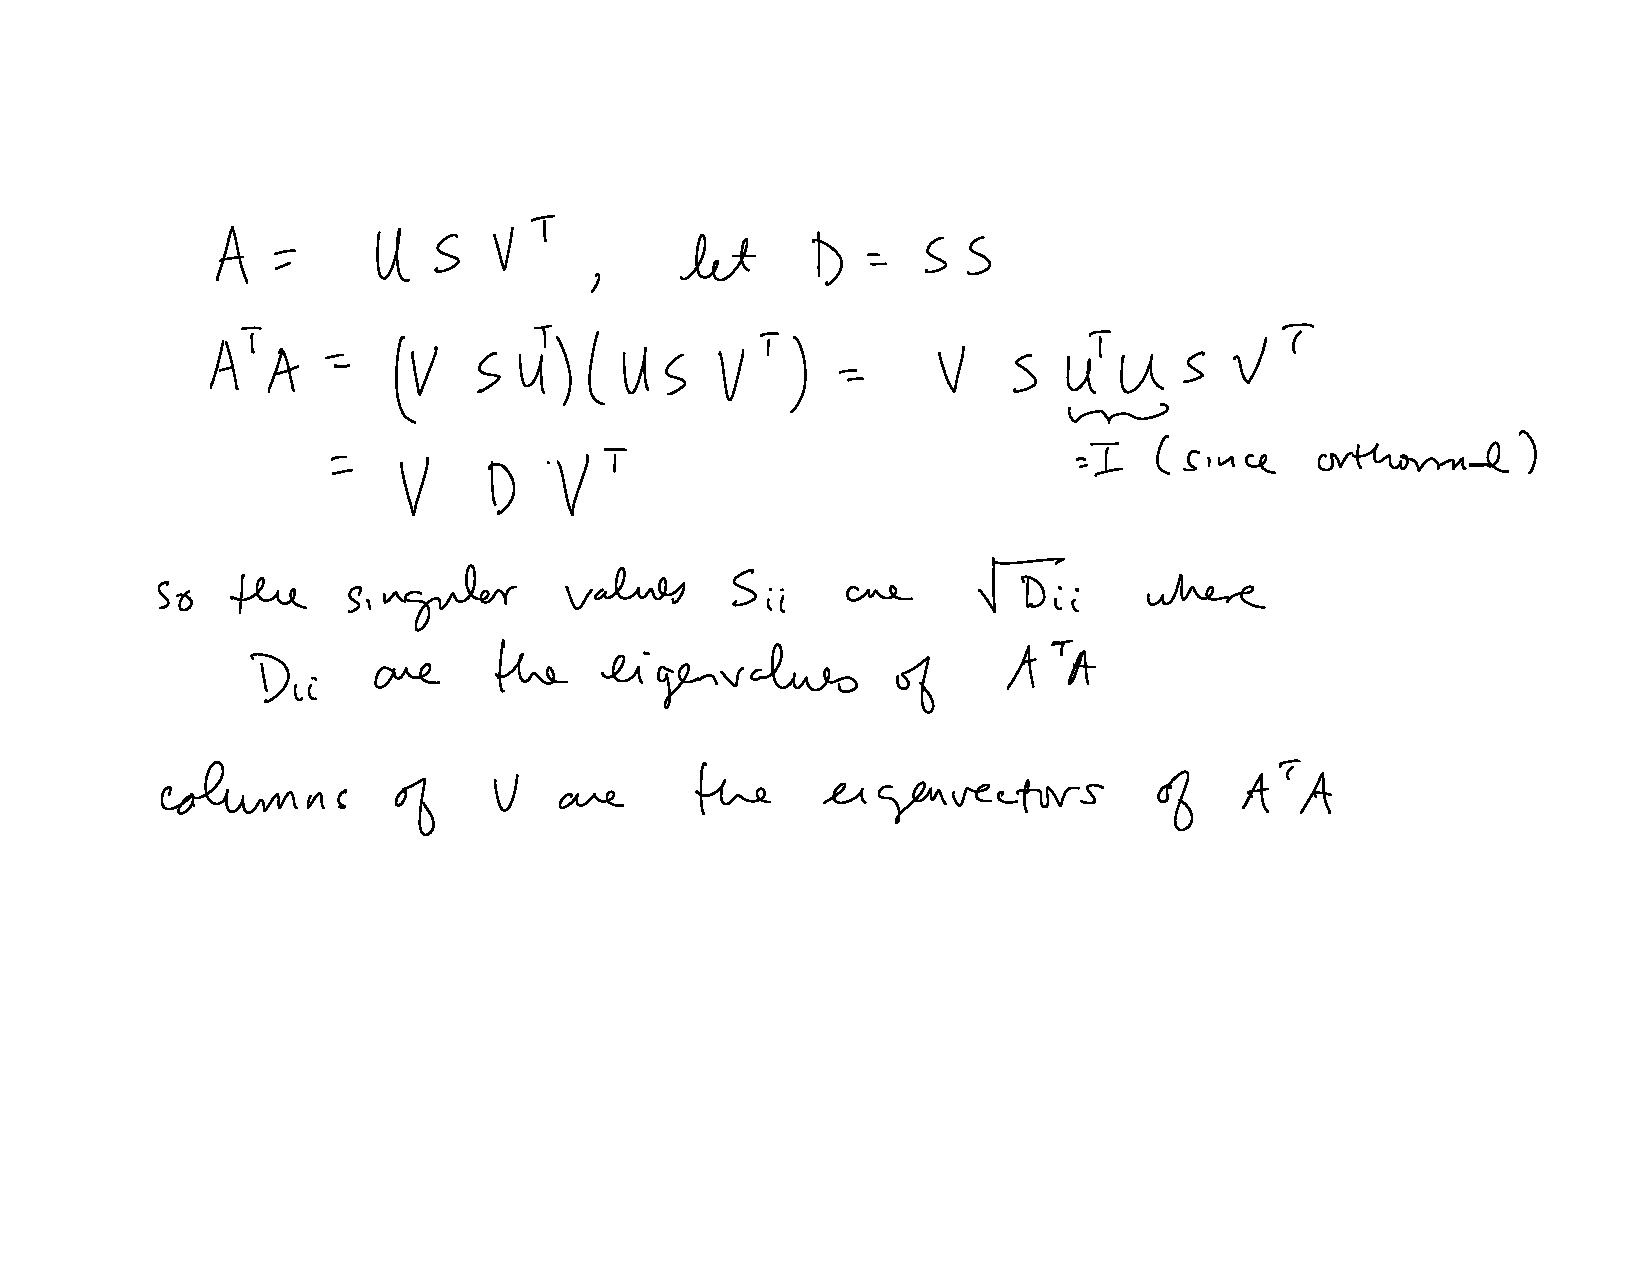
\includegraphics[height=2in]{svd-reln-eigen}
\end{center}

\end{frame}
%===========================================================

%===========================================================
\begin{frame}
  \frametitle{Using SVD to do PCA}

\begin{center}
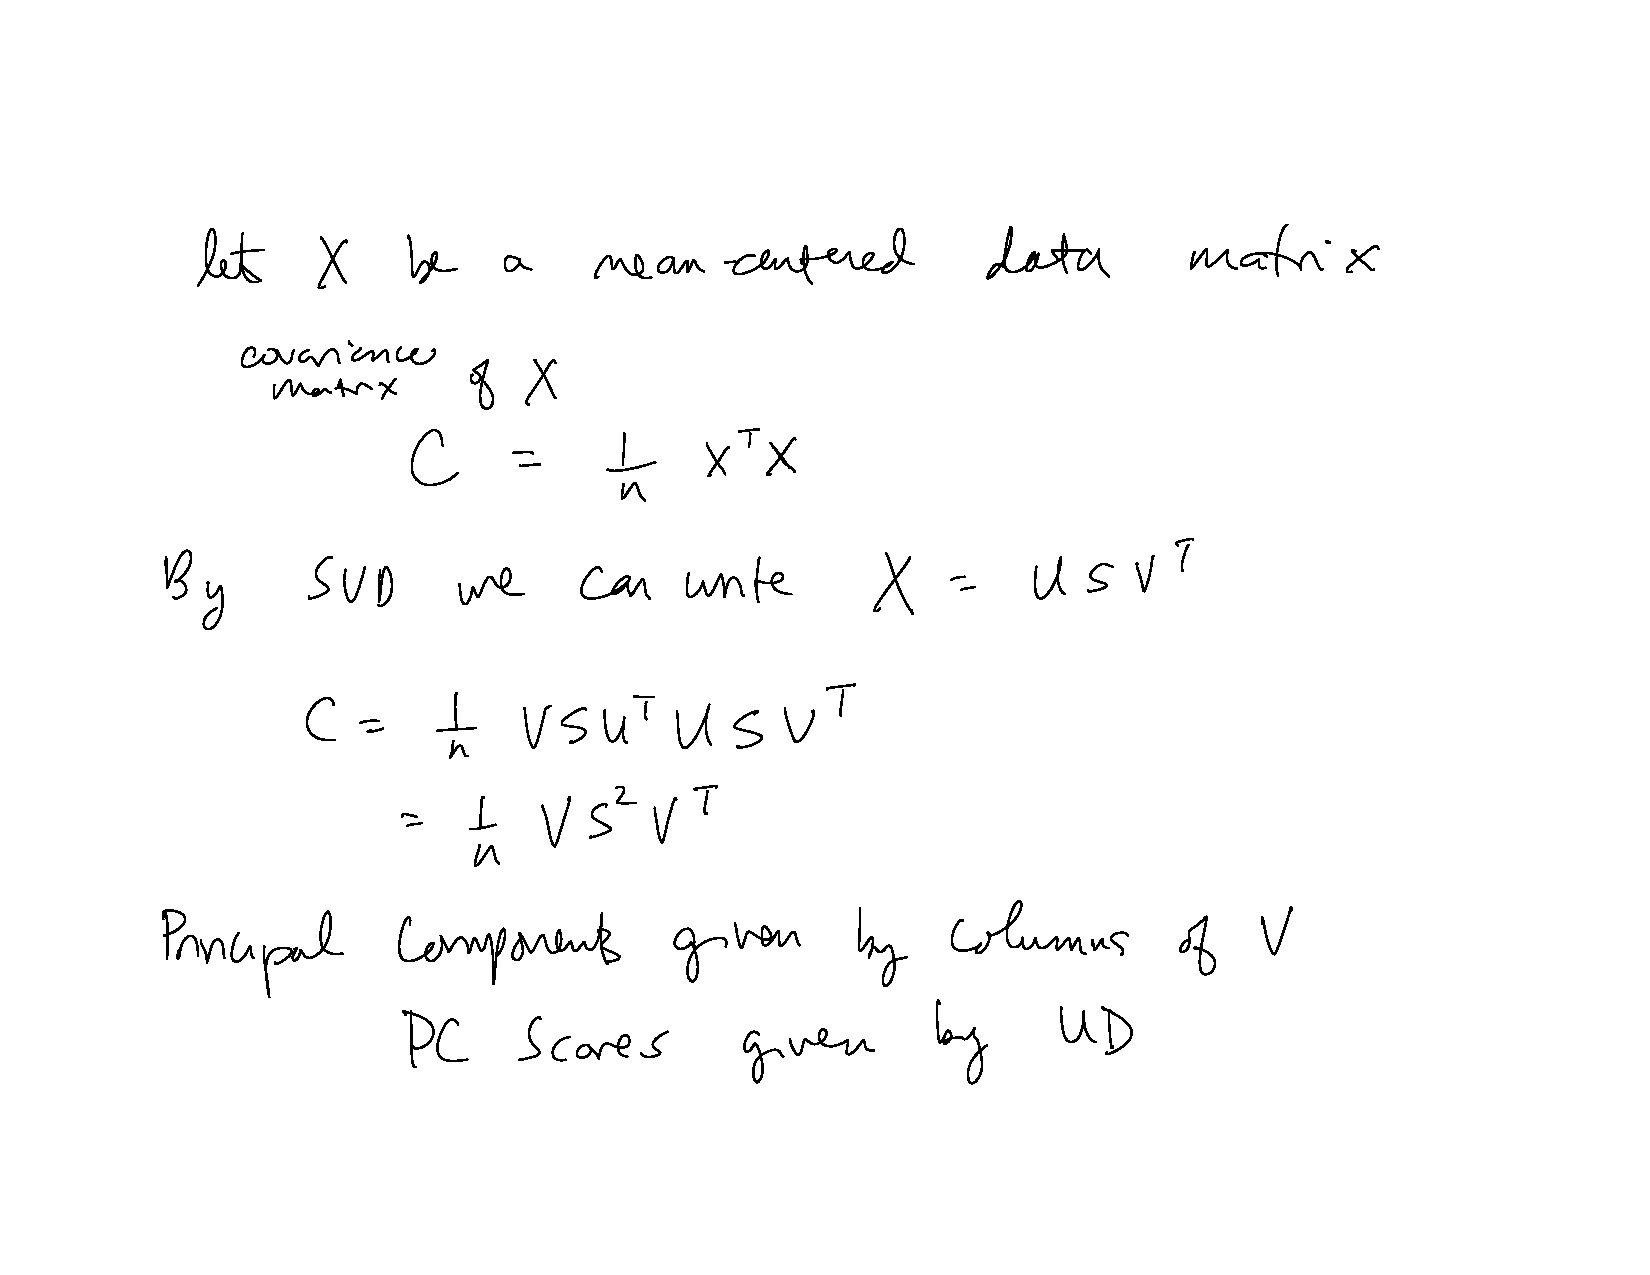
\includegraphics[height=2.5in]{svd-pca}
\end{center}

\end{frame}

%===========================================================
\begin{frame}
  \frametitle{Another Way of Thinking about SVD}


\begin{center}
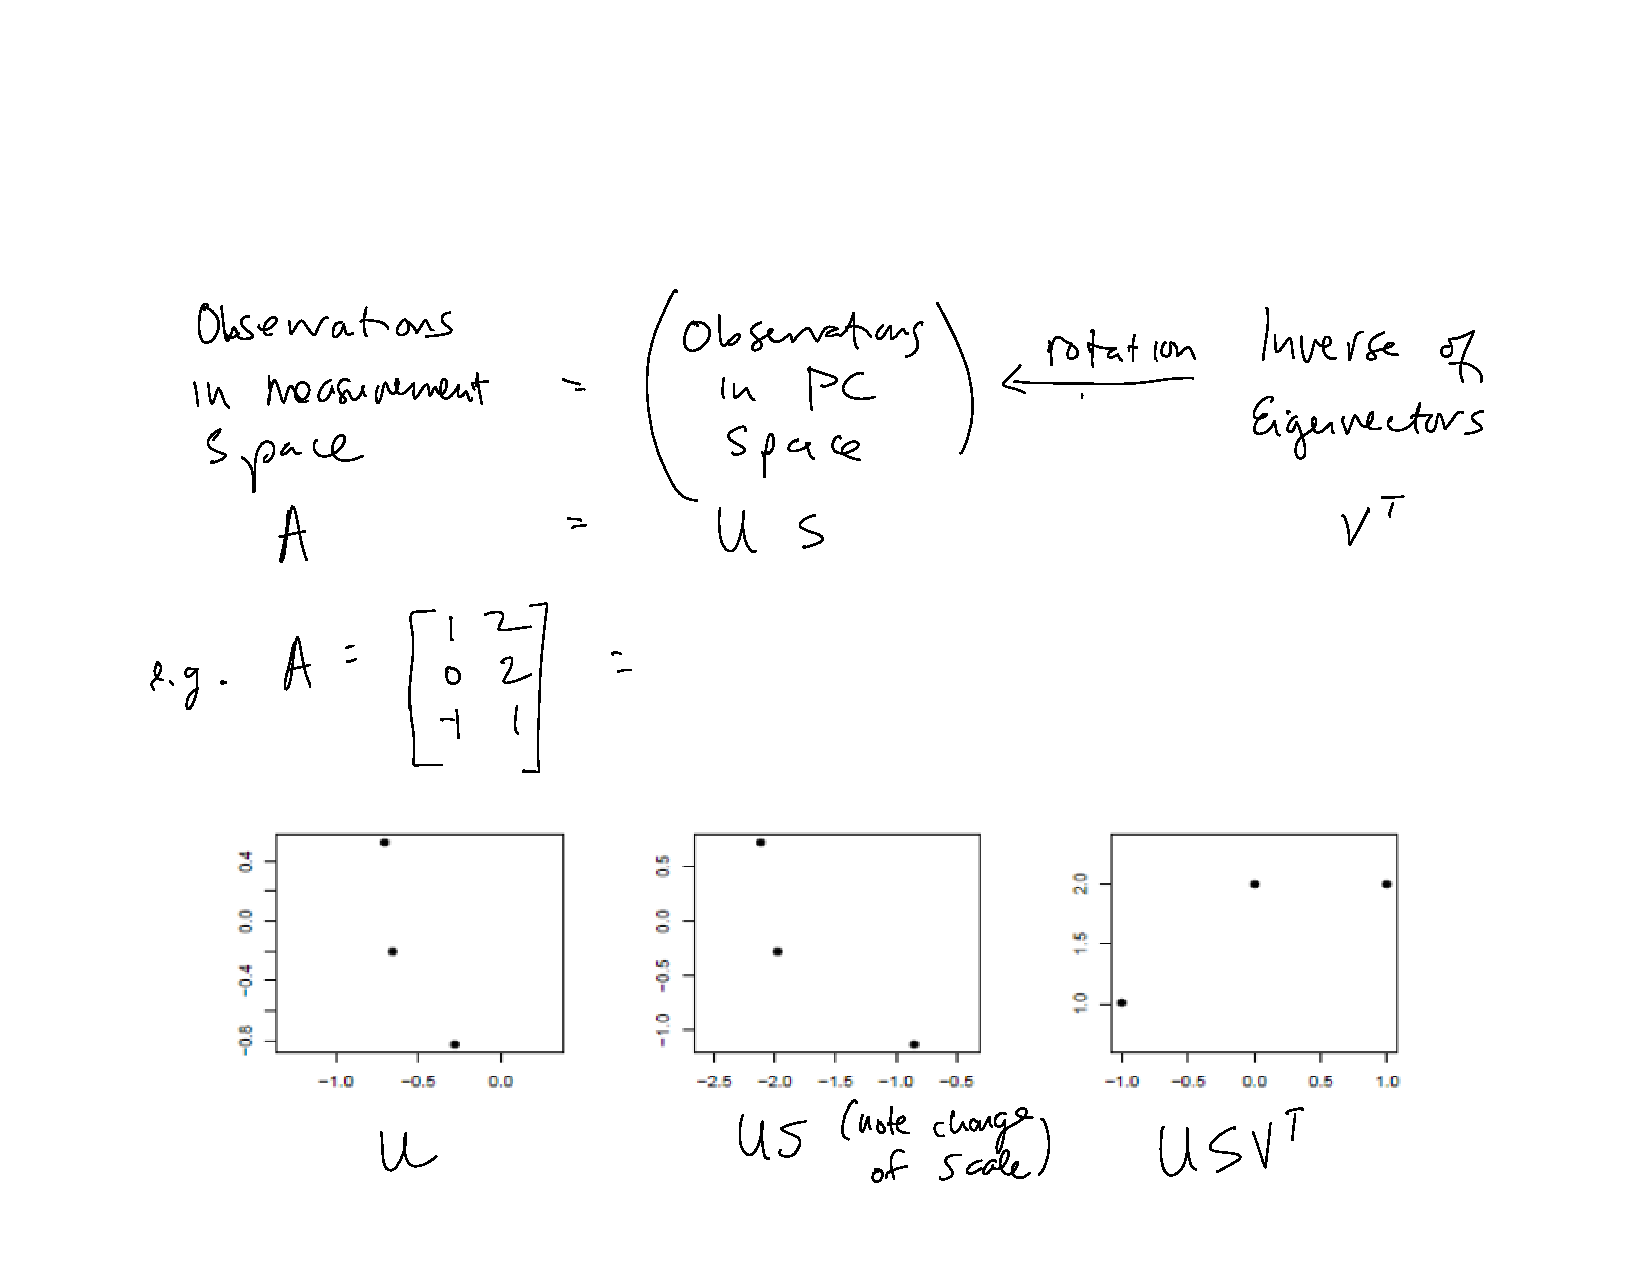
\includegraphics[height=2.5in]{svd-another-view}
\end{center}

\end{frame}

%===========================================================


%===========================================================
\begin{frame}
  \frametitle{Applications of SVD}

\begin{itemize}
\item Pseudoinverse of an arbirary matrix
\item Matrix approximation
\item Motivates the Biplot and Correspondence Analysis
\end{itemize}

\end{frame}
%===========================================================


%===========================================================
\begin{frame}
  \frametitle{Pseudoinverse via SVD}

The pseudoinverse of a matrix is a generalization of the concept of a matrix inverse. Only square matrices have a matrix inverse; the pseudoinverse applies to an arbitrary $n \times p$ matrix.

\smallskip
Given an $n \times p$ matrix $\Mtx{A}$ find matrix $\PsInv{A}$ such that:

\begin{eqnarray*}
\Mtx{A} \PsInv{A} \Mtx{A} & = & \Mtx{A} \\
\PsInv{A} \Mtx{A} \PsInv{A} & = & \PsInv{A}\\
(\Mtx{A} \PsInv{A})^T & = & \Mtx{A} \PsInv{A}\\
(\PsInv{A} \Mtx{A})^T & = & \PsInv{A} \Mtx{A}
\end{eqnarray*}

\smallskip
Moore-Penrose Inverse via SVD:

\begin{eqnarray*}
\text{if}\ \Mtx{A} &=& \Mtx{U}\Mtx{S}\Mtx{V}^T \\
\PsInv{A} &=& \Mtx{V} \PsInv{S}  \Mtx{U}^T
\end{eqnarray*}

where \PsInv{S} has the reciprocal of non-zero elements of S.

\end{frame}
%===========================================================

%===========================================================
\begin{frame}
  \frametitle{SVD for Matrix Approximation}

If $ \Mtx{A} = \Mtx{U} \Mtx{S} \Mtx{V}^T $
then the optimal (least-squares) $k$-dimensional approximation of \Mtx{A} (where $ k < \rank(\Mtx{A})$) is given by:
$$ \tilde{\Mtx{A}} = \Mtx{U}\Mtx{S}^{\thinstar} \Mtx{V}^T$$ 

where:
\begin{eqnarray*}
\Mtx{S}_{ii}^{\thinstar} &=& \Mtx{S}_{ii} \text{ for } i \leq k\\
\Mtx{S}_{ii}^{\thinstar} &=& 0 \text{ for } i > k\\
\end{eqnarray*}

\end{frame}
%===========================================================


%===========================================================
\begin{frame}
  \frametitle{Biplots}


\begin{center}
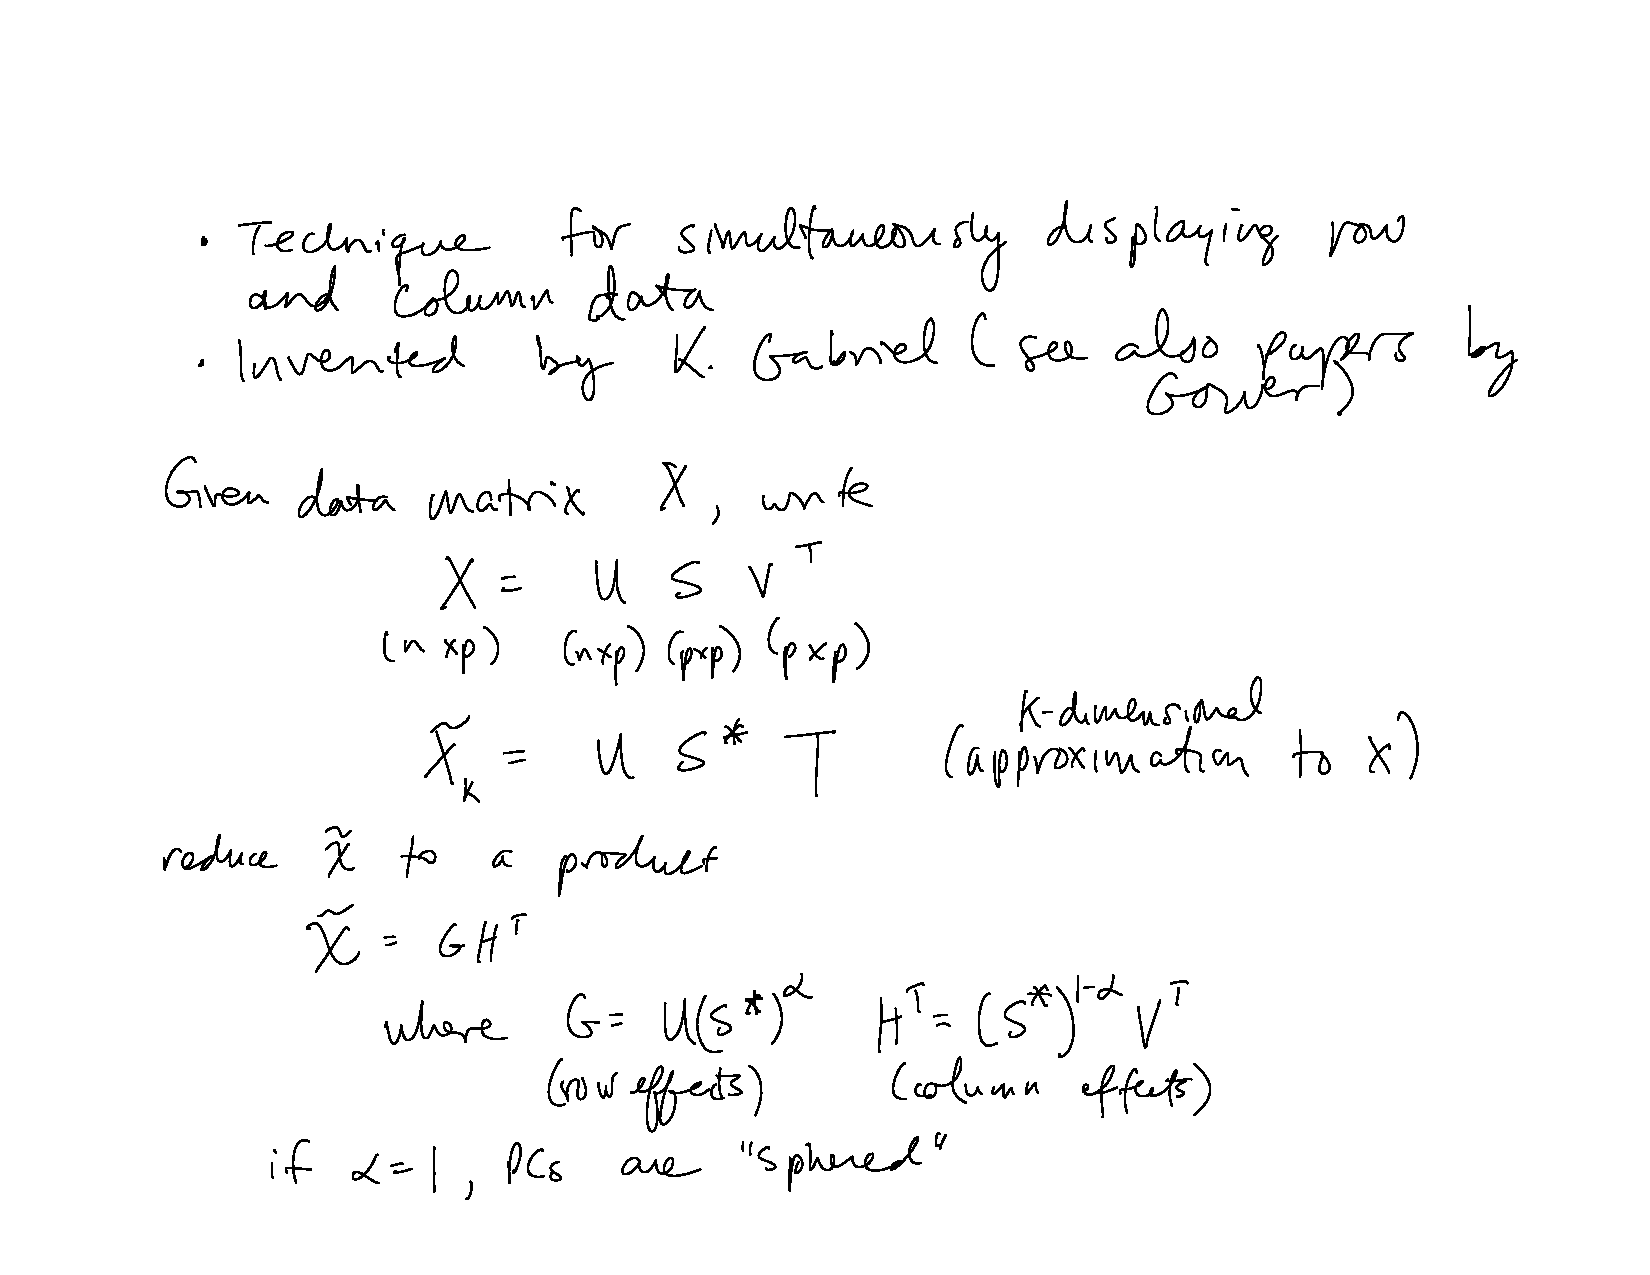
\includegraphics[height=2.75in]{about-biplots}
\end{center}

\end{frame}

%===========================================================

%===========================================================
\begin{frame}
  \frametitle{Biplots}

\begin{eqnarray*}
\Mtx{G} &=& \Mtx{U}(\Mtx{S}^{\thinstar})^{\alpha} \text{ (row effects) } \\
\Mtx{H}^T &=& (\Mtx{S}^{\thinstar})^{1-\alpha} \Mtx{V}^T \text{ (columns effects) }
\end{eqnarray*}

Different choices of $\alpha$ emphasize different relationships in the data.

\begin{itemize}
\item \Red{$\alpha = 0$}, column-metric preserving biplot; optimally approximates variance-covariance structure. Cosine of angles between vectors approximate correlations; distances between points approximate Mahalanobis distance ( ``correlation biplot'')
\item \Red{$\alpha = 1$}, row-metric preserving biplot; optimally approximates Euclidean distances among observations. Coordinates of observations correspond to PC scores; coordinates of variables correspond to eigenvector coefficients (``distance biplot'')
\item \Red{$\alpha = 0.5$},  optimally approximates observational values (``symmetric biplot'')
\end{itemize}

\end{frame}

%===========================================================

%===========================================================
\begin{frame}
  \frametitle{Biplots, Example}


\begin{center}
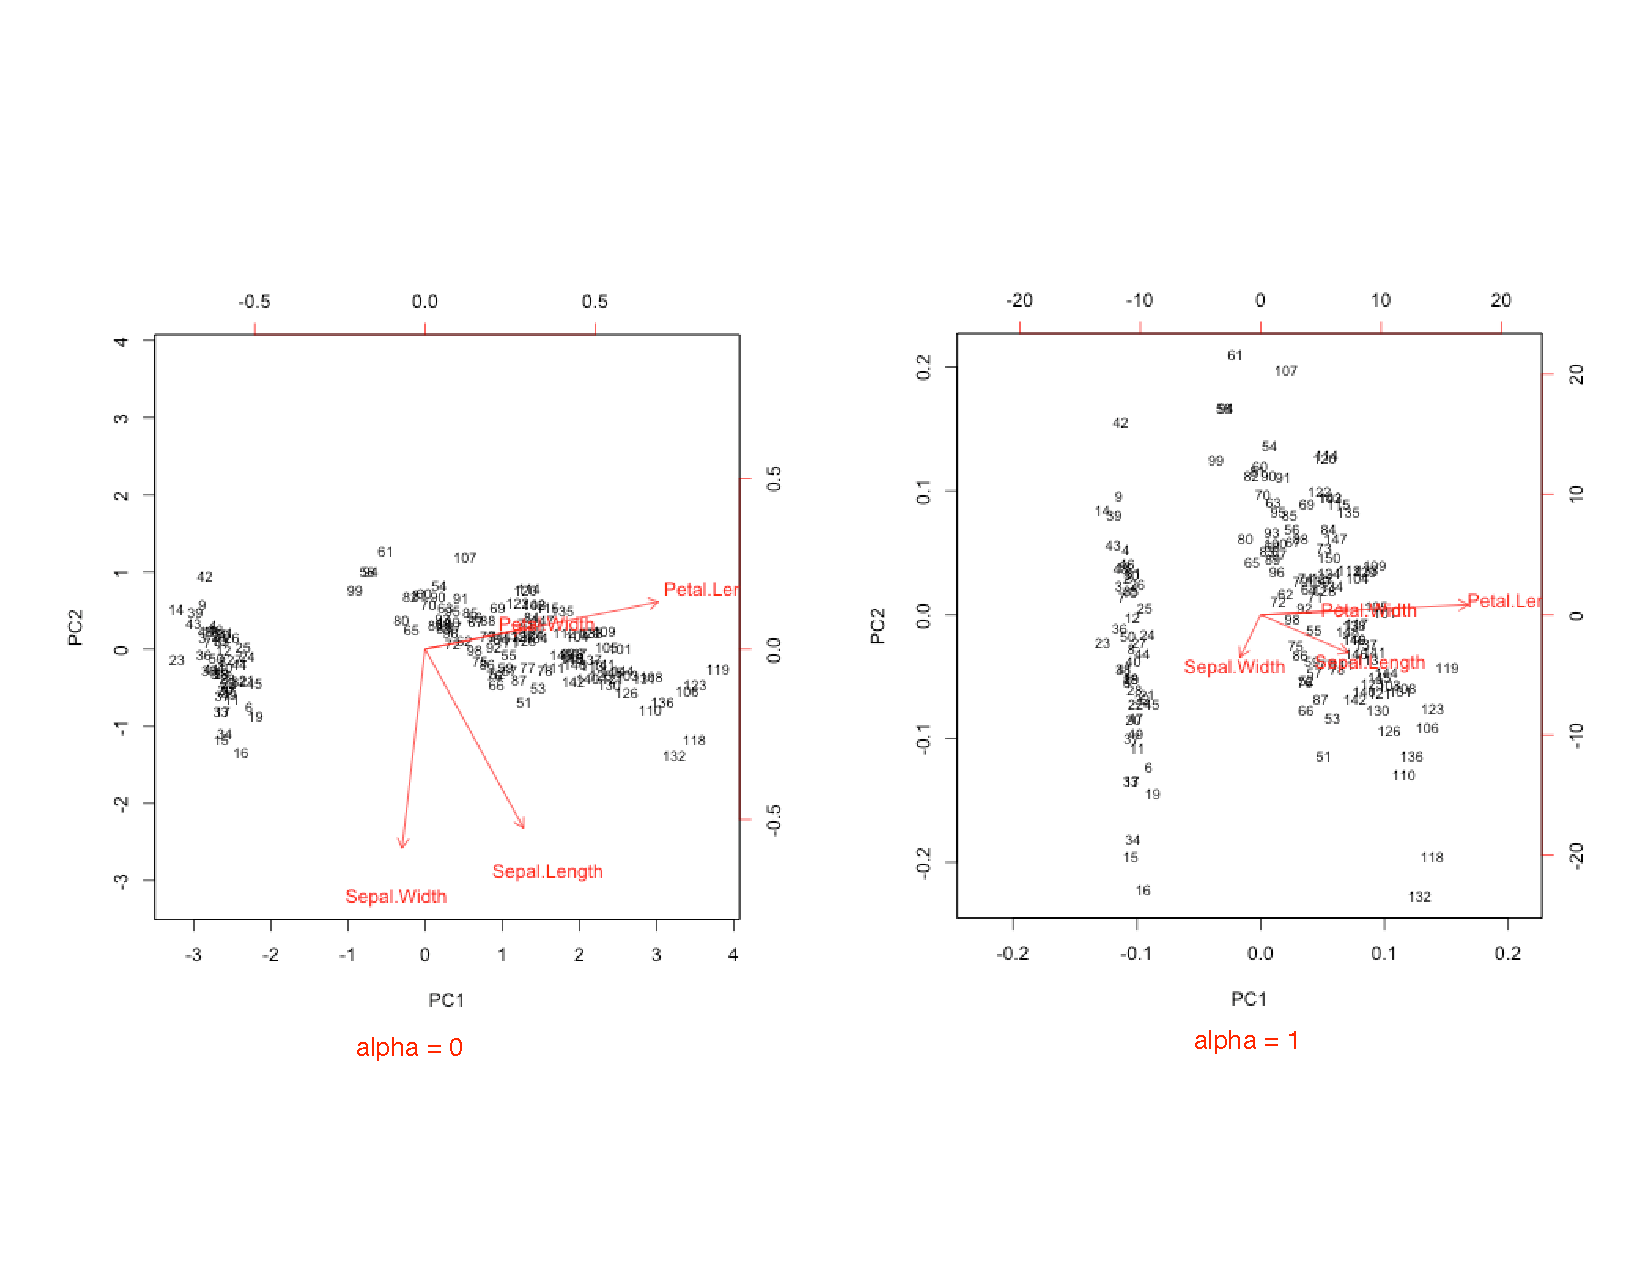
\includegraphics[height=2.5in]{iris-biplots2}

{\footnotesize Anderson's famous iris data set.}
\end{center}


\end{frame}

%===========================================================


%===========================================================
\begin{frame}
  \frametitle{Biplots, Example II}
\begin{itemize}
\item Observations drawn as points in space of PCs
\item Variables drawn as vectors in PC space
\end{itemize}

\begin{center}
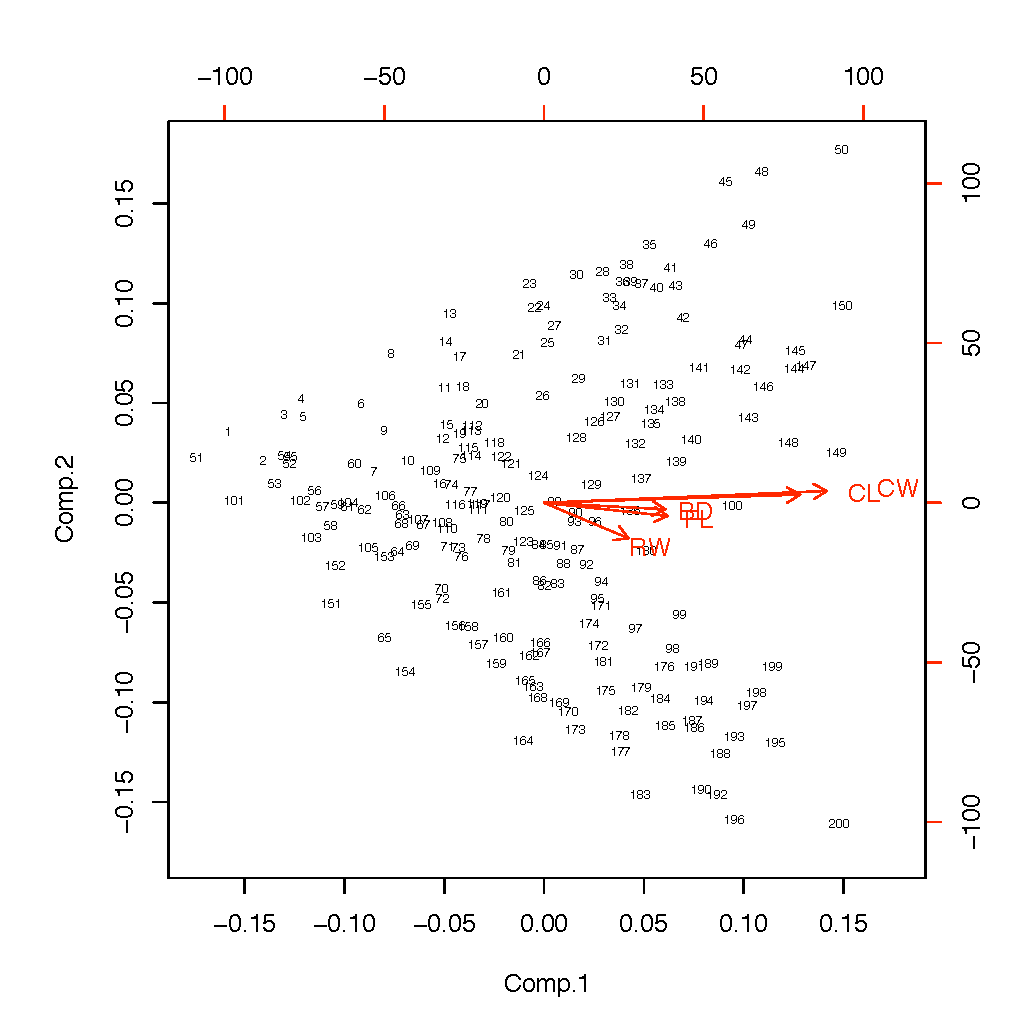
\includegraphics[height=2.25in]{crab-biplot}

{\footnotesize Biplot ($\alpha=1$) for dataset of five morphological measurements on crabs.}
\end{center}


\end{frame}

%===========================================================



% 
% %===========================================================
% \begin{frame}
%   \frametitle{Correspondence Analysis}
% 
% 
% \begin{center}
% \includegraphics[height=2.75in]{about-correspondence1}
% \end{center}
% 
% \end{frame}
% 
% %===========================================================
% 
% \begin{frame}
%   \frametitle{Correspondence Analysis II}
% 
% 
% \begin{center}
% \includegraphics[height=2.75in]{about-correspondence2}
% \end{center}
% 
% \end{frame}
% 
% %===========================================================
% 
% 
% \begin{frame}
%   \frametitle{Solving the Correspondence Analysis Problem}
% 
% 
% \begin{center}
% \includegraphics[height=2.75in]{solving-correspondence1}
% \end{center}
% 
% \end{frame}
% 
% %===========================================================
% 
% 
% \begin{frame}
%   \frametitle{Solving CA, cont.}
% 
% 
% \begin{center}
% \includegraphics[height=2.75in]{solving-correspondence2}
% \end{center}
% 
% \end{frame}
% 
% %===========================================================
% 
% \begin{frame}
%   \frametitle{Visualizing a Correspondence Analysis}
% 
% Results of correspondence analysis often depicted as a biplot!
% 
% 
% 
% \begin{center}
% \includegraphics[height=0.75in]{correspondence-table}
% 
% \includegraphics[height=2in]{correspondence-biplot}
% \end{center}
% 
% \end{frame}
% 
% %===========================================================

\end{document}


%===========================================================
\begin{frame}
  \frametitle{XXX}

\end{frame}
%===========================================================
